%%  CHAPTER 3
%%  Understanding the README Framework: Representation Learning
%%  by Fairness-Aware Disentangling Method
%%
%%  Based on:  Park et al., arXiv:2007.03775v1 (2020)
%%  Written for the CSC-391 Technical Communication report
%%  "Ethics in AI: Emphasis on Fairness" — Group 7, IITR 2026
%% ============================================================
\setlength{\headheight}{14.5pt}
\addtolength{\topmargin}{-2.5pt}

\chapter{README Framework: Fair Representation Learning Through Disentanglement}
\label{ch:readme}



%% ---- Declaration of Contributions ----------------------------
\vspace{0.5em}
\noindent\rule{\textwidth}{0.4pt}
\textbf{Declaration of Contributions:}
\begin{itemize}[leftmargin=*,noitemsep]
\item \textbf{Pradyuman Singh Shekhawat} — Reviewed key concepts including Variational Autoencoders,
      Total Correlation, and the disentanglement loss derivation; wrote
      Sections~\ref{sec:readme-motivation}--\ref{sec:readme-disentanglement}. Studied and explained the FD-VAE architecture,
      the decorrelation module, and the downstream classification network;
      wrote Sections~\ref{sec:readme-architecture}--\ref{sec:readme-downstream}.
\item \textbf{Vishesh Gupta} — Interpreted the fairness metrics and experimental results;
      wrote Sections~\ref{sec:readme-results}.
\end{itemize}
\noindent\rule{\textwidth}{0.4pt}
\vspace{1em}

% ----------------------------------------------------------------
\section{Motivation and Problem Setting}
\label{sec:readme-motivation}
% ----------------------------------------------------------------

One of the most natural entry-points for tackling bias in machine learning is to attack the problem at
the level of \emph{representation}: if the feature vector that a model learns contains no information
about a sensitive attribute, then any classifier built on top of that vector cannot discriminate on
the basis of that attribute. This idea is the backbone of the \textbf{README} (REpresentation learning
by fairness-Aware Disentangling MEthod) paper by Park \emph{et al.}~\cite{park2020readme}.

Formally, let us denote the observed data by $\mathcal{X} = \{x_1, \ldots, x_n\}$, the target
attribute labels by $\mathcal{Y}_t = \{y_{t_1}, \ldots, y_{t_n}\}$, and the protected attribute
labels by $\mathcal{Y}_p = \{y_{p_1}, \ldots, y_{p_n}\}$. A protected attribute is any characteristic
such as \emph{gender}, \emph{age}, or \emph{race} on which individuals ought not to be
discriminated against. A target attribute is the quantity the downstream classifier is actually
supposed to predict, e.g., whether a face is \emph{attractive} or whether the hair is
\emph{wavy}. The challenge is that in real-world datasets, target and protected attributes are
often statistically correlated --- for example, the ``attractive'' label in the CelebA dataset is
influenced by the gender distribution in the data~\cite{park2020readme}.

\subsection{Limitation of Earlier Disentanglement Approaches}
\label{ssec:readme-ffvae-limitation}

Prior to README, the state-of-the-art approach for fair representation learning via disentanglement was
\textbf{FFVAE} (Flexibly Fair Variational AutoEncoder) by Creager~\emph{et al.}~\cite{creager2019ffvae}.
FFVAE partitions the latent space into two parts:
\begin{itemize}
    \item \emph{Sensitive latents}: latent variables trained to be highly informative about the
          protected attribute; and
    \item \emph{Non-sensitive latents}: latent variables trained to be independent of the sensitive
          latents.
\end{itemize}
During downstream classification, only the non-sensitive latents are used, with the reasoning that
this excludes all protected-attribute information from the prediction pipeline.

Park~\emph{et al.} identify a fundamental flaw in this two-way split. Because real-world attributes
are correlated, the sensitive latents end up capturing \emph{both} protected-attribute information
\emph{and} some target-attribute information. When these latents are excluded for fairness, useful
discriminative signal for the target task is discarded along with the demographic information. The
authors demonstrate this empirically: when they perform downstream classification using each
subspace independently on the CelebA dataset (target attribute = \emph{attractive}, protected
attribute = \emph{male}), the sensitive latents actually produce \emph{higher} accuracy on the
target attribute than the non-sensitive latents (67.4\% vs 62.7\%), revealing that excluding them
comes at an unnecessary accuracy cost.

This observation motivates the central design choice of README: the latent space should be split into
\emph{three} independent subspaces, not two --- separating target information, protected information,
and the \emph{shared} information predictive of both into its own dedicated slot.

\begin{figure}[htbp]
    \centering
    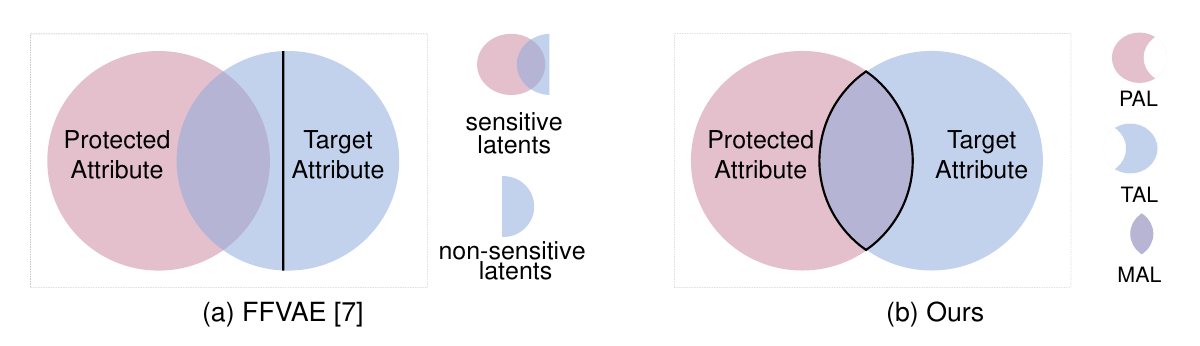
\includegraphics[width=\textwidth]{figures/readme-motivation.png}
    \caption{
        Motivation for fairness-aware disentanglement.
        (a) Prior methods (e.g., FFVAE) mix target and protected information, causing loss of useful features.
        (b) README separates them into TAL, PAL, and MAL, isolating shared information without harming performance.
    }
    \label{fig:readme-motivation}
\end{figure}
% ----------------------------------------------------------------
\section{Overview of the FD-VAE Architecture}
\label{sec:readme-architecture}
% ----------------------------------------------------------------

The README framework is built around a model called the \textbf{Fairness-aware Disentangling
Variational AutoEncoder (FD-VAE)}. At a high level, the FD-VAE is a VAE extended with two additional
components: a discriminator for encouraging disentanglement across the three subspaces, and a
decorrelation module that explicitly specifies \emph{which type} of information should reside in
each subspace.

The architecture operates in two stages:
\begin{enumerate}
    \item \textbf{Representation Learning Stage}: The FD-VAE (encoder + decoder + discriminator +
          decorrelation module) is trained jointly to produce a well-disentangled and decorrelated
          latent space.
    \item \textbf{Downstream Classification Stage}: The encoder is frozen, and a lightweight
          classification network is trained on the learned latent variables to predict the target
          attribute in a fairness-preserving manner.
\end{enumerate}

\begin{figure}[htbp]
    \centering
    % Replace the placeholder with the actual architecture figure from the paper
    % or the one recreated in Chapter figures/fdvae_architecture.pdf
    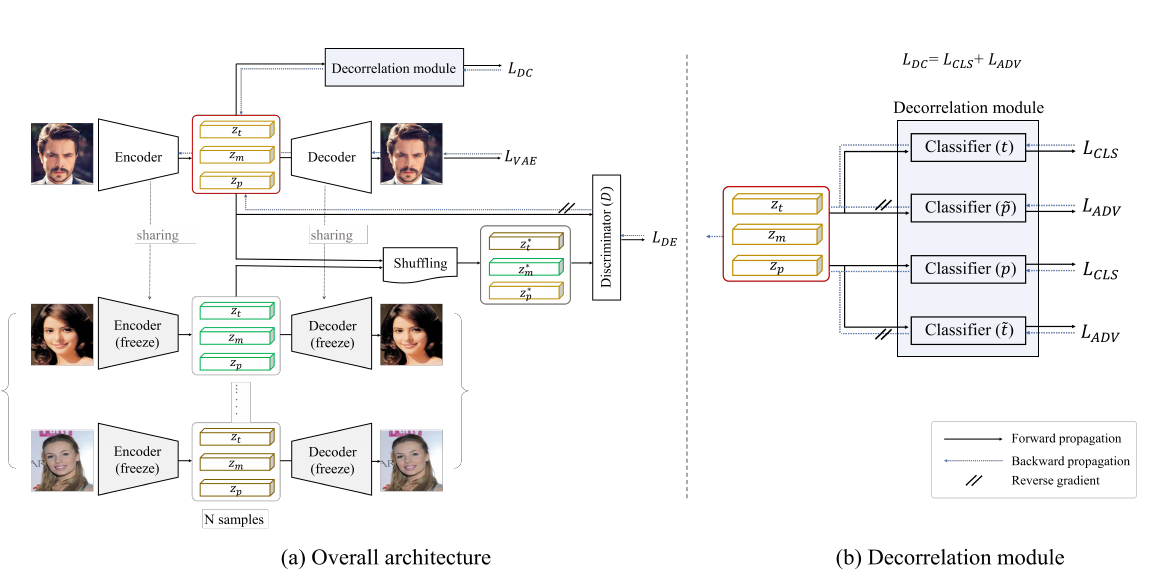
\includegraphics[width=\linewidth]{figures/readme-architecture.png}
    \caption{%
        Full architecture of the Fairness-aware Disentangling VAE (FD-VAE).
        Source: adapted from Park \emph{et al.}~\cite{park2020readme}.
    }
    \label{fig:fdvae-overview}
\end{figure}

\subsection{The Three Latent Subspaces}

The encoder $q_\Phi(z \mid x)$ maps an input image to three independent latent subspaces:

\begin{description}
    \item[Target Attribute Latent (TAL), $z_t$.]  This subspace is trained to carry only the
          information that is predictive of the target attribute $y_t$. During representation learning
          it receives a supervised classification signal for $y_t$ and an adversarial signal that
          prevents it from leaking protected-attribute information.

    \item[Protected Attribute Latent (PAL), $z_p$.]  Symmetrically, this subspace is trained to
          contain only protected-attribute information $y_p$. Because it carries the demographic
          signal, it is \emph{excluded entirely} from the downstream classification pipeline to ensure
          that the final predictor cannot use demographic information.

    \item[Mutual Attribute Latent (MAL), $z_m$.]  This is the key novelty of README. In real datasets
          there exists information that is predictive of \emph{both} $y_t$ and $y_p$ simultaneously
          (e.g., facial structure features that correlate with both attractiveness and gender). If this
          shared information were forced into either TAL or PAL, it would violate the decorrelation
          objective. MAL provides a dedicated ``overflow'' subspace for this information. During
          downstream classification, the protected-attribute signal in MAL is stripped away before
          MAL's remaining content is used to augment the classification.
\end{description}

In all experiments, each subspace is set to 20 dimensions, for a total latent dimension of 60.

% ----------------------------------------------------------------
\section{The Variational Autoencoder Objective}
\label{sec:readme-vae}
% ----------------------------------------------------------------

The encoder and decoder follow the standard VAE formulation of Kingma and
Welling~\cite{kingma2014vae}. The encoder outputs mean and variance parameters
$(\mu, \sigma) = q_\Phi(x)$, from which latent codes are drawn via the reparameterisation trick:
\[
    z \sim \mathcal{N}\!\left(\mu_{q_\Phi}(x),\, \sigma_{q_\Phi}(x)\right).
\]
The VAE objective is to maximise the Evidence Lower Bound (ELBO):
\begin{equation}
    L_\text{VAE} = \sum_{i=1}^{n}
        \mathbb{E}_{q_\Phi(z_t, z_p, z_m \mid x_i)}\!\left[
            \log p_\Theta(x_i \mid z_t, z_p, z_m)
        \right]
        - \mathrm{KL}\!\left[
            q_\Phi(z_t, z_p, z_m \mid x_i)
            \,\|\,
            p(z_t, z_p, z_m)
        \right].
    \label{eq:vae-elbo}
\end{equation}
The first term is the \emph{reconstruction loss}: the decoder $p_\Theta$ tries to faithfully
reconstruct each input from the concatenated latent codes $(z_t, z_p, z_m)$. The second term
is the \emph{KL regularisation loss}: it encourages the posterior $q_\Phi$ to remain close to
the standard Gaussian prior $p(z) = \mathcal{N}(0, I)$, which acts as a regulariser and ensures
the latent space has good coverage.

% ----------------------------------------------------------------
\section{Disentanglement Loss via Total Correlation}
\label{sec:readme-disentanglement}
% ----------------------------------------------------------------

The VAE objective alone does not enforce that the three subspaces $z_t$, $z_p$, and $z_m$ are
\emph{mutually independent}. Mutual independence between subspaces is formalised using the
\textbf{Total Correlation (TC)}~\cite{watanabe1960tc}, which is the KL divergence between the joint
distribution and the product of its marginals:
\begin{equation}
    L_\text{DE} = \mathrm{KL}\!\left[
        q_\Phi(z_t, z_p, z_m)
        \,\Big\|\,
        \prod_{j \in S} q_\Phi(z_j)
    \right]
    = \mathbb{E}_{q_\Phi(z_t, z_p, z_m)}\!\left[
        \log \frac{q_\Phi(z_t, z_p, z_m)}{\prod_{j \in S} q_\Phi(z_j)}
    \right],
    \label{eq:tc}
\end{equation}
where $S = \{t, p, m\}$. Minimising the Total Correlation forces the three subspaces to become
maximally independent of each other, which is the formal definition of disentanglement.

\subsection{Adversarial Approximation of the Discriminator}

Directly computing the log-density ratio in Equation~\eqref{eq:tc} is intractable. Following the
approach of Kim and Mnih~\cite{kim2018factorVAE}, the log-density ratio is approximated by training
a discriminator $D$ to classify between \emph{real samples} (drawn from the joint $q_\Phi(z_t, z_p, z_m)$)
and \emph{fake samples} $z^* = [z_t^*; z_p^*; z_m^*]$ generated by independently shuffling each
subspace within a mini-batch:
\begin{equation}
    L_\text{DE} \approx \mathbb{E}_{q_\Phi(z_t, z_p, z_m)}\!\left[
        \log \frac{D(z_t, z_p, z_m)}{1 - D(z_t, z_p, z_m)}
    \right].
    \label{eq:tc-approx}
\end{equation}
The discriminator is trained separately to classify real vs.\ fake by minimising:
\begin{equation}
    L_D = -\mathbb{E}_{q_\Phi(z_t, z_p, z_m)}\!\left[
        \log D(z_t, z_p, z_m) + \log\!\left(1 - D(z_t^*, z_p^*, z_m^*)\right)
    \right].
    \label{eq:disc-loss}
\end{equation}
The encoder $q_\Phi$ is simultaneously trained to fool the discriminator, which drives the Total
Correlation toward zero and therefore encourages independence between the three subspaces.

% ----------------------------------------------------------------
\section{Decorrelation Loss}
\label{sec:readme-decorrelation}
% ----------------------------------------------------------------

The disentanglement loss ensures that the three subspaces are \emph{statistically independent}, but
it says nothing about \emph{which information goes where}. The decorrelation loss $L_\text{DC}$
takes over this role: it provides explicit supervision to ensure that $z_t$ contains target
attribute information, $z_p$ contains protected attribute information, and each is purged of the
other's signal.

The decorrelation loss is composed of two terms:
\begin{equation}
    L_\text{DC} = \beta L_\text{CLS} + \gamma L_\text{ADV},
    \label{eq:dc}
\end{equation}
where $\beta$ and $\gamma$ are hyperparameters (set to 5 and 10, respectively, in all experiments).

\subsection{Classification Loss \texorpdfstring{$L_\text{CLS}$}{L\_CLS}}
\label{ssec:lcls}

The classification loss provides direct supervision to assign the correct information to the correct
subspace. It minimises cross-entropy for predicting the target label $y_t$ from $z_t$, and for
predicting the protected label $y_p$ from $z_p$:
\begin{equation}
    L_\text{CLS} = -\sum_{i=1}^{n}
        \mathbb{E}_{q_\Phi(z_t, z_p, z_m \mid x_i)}\!\Big[
            \log p_t(y_{t_i} \mid z_t) + \log p_p(y_{p_i} \mid z_p)
        \Big],
    \label{eq:lcls}
\end{equation}
where $p_t$ and $p_p$ are lightweight classifiers (single fully-connected layers) trained to predict the
target and protected attributes from their respective subspaces.

\subsection{Adversarial Loss \texorpdfstring{$L_\text{ADV}$}{L\_ADV}}
\label{ssec:ladv}

The classification loss alone is not enough: it pushes the correct information \emph{into} each
subspace but does not actively remove unwanted cross-information. The adversarial loss does this by
training two adversarial classifiers $\tilde{p}$ (predicting $y_p$ from $z_t$) and $\tilde{t}$
(predicting $y_t$ from $z_p$), and using \emph{reverse gradients} to force the encoder to make these
classifiers fail:
\begin{equation}
    L_\text{ADV} = \max_{\tilde{t},\, \tilde{p}}\;
        \min_{\Phi}\; \sum_{i=1}^{n}
        \mathbb{E}_{q_\Phi(z_t, z_p, z_m \mid x_i)}\!\Big[
            \log p_{\tilde{p}}(y_{p_i} \mid z_t) + \log p_{\tilde{t}}(y_{t_i} \mid z_p)
        \Big].
    \label{eq:ladv}
\end{equation}
The minimax structure is crucial: the adversarial classifiers $\tilde{p}$ and $\tilde{t}$ are
trained to \emph{maximise} their ability to predict cross-attribute labels, while the encoder
$q_\Phi$ is trained to \emph{minimise} this ability. This creates a game that drives protected-attribute
information out of $z_t$ and target-attribute information out of $z_p$.

\subsection{The Role of the Mutual Attribute Latent in Decorrelation}

A key subtlety is what happens to information that is genuinely predictive of \emph{both} attributes
simultaneously. Forcing this information into either $z_t$ or $z_p$ would increase $L_\text{ADV}$ in
either direction. The MAL $z_m$ acts as a pressure valve: the disentanglement loss $L_\text{DE}$
indirectly encourages this shared information to migrate into $z_m$, because placing it there
satisfies both the independence constraint and keeps $L_\text{ADV}$ low. No additional explicit
mapping is applied to $z_m$ during representation learning.

\subsection{Total Objective for Stage 1}

The full representation learning objective that the FD-VAE maximises is:
\begin{equation}
    L_\text{TOTAL} = L_\text{VAE} - \alpha L_\text{DE} - L_D - L_\text{DC},
    \label{eq:total}
\end{equation}
where $\alpha$ is a hyperparameter controlling the strength of the disentanglement
objective ($\alpha = 50$ in all experiments). The negative signs on $L_\text{DE}$ and $L_D$ reflect
the fact that the encoder is trained to \emph{minimise} Total Correlation (thus maximise the negated
discriminator objective), while the discriminator $D$ is trained separately to minimise $L_D$.

% ----------------------------------------------------------------
\section{Downstream Classification Network}
\label{sec:readme-downstream}
% ----------------------------------------------------------------

Once Stage 1 training is complete, the encoder weights are frozen and the downstream classification
network is trained to predict $y_t$ in a fair manner.

\paragraph{Excluding PAL.}
The Protected Attribute Latent $\hat{z}_p$ is dropped entirely. Because the decorrelation objective
has already separated all target-attribute information out of $\hat{z}_p$, this exclusion does not
hurt target-prediction accuracy while guaranteeing that the final classifier has no access to
demographic information.

\paragraph{Sanitising MAL.}
The Mutual Attribute Latent $\hat{z}_m$ still carries some residual protected-attribute signal (since
it holds the shared information). A single fully connected layer $f$ is applied to $\hat{z}_m$ to
produce a transformed representation $z_n$. An adversarial protected-attribute classifier $\tilde{d}$
is trained to extract demographic information from $z_n$ via reverse gradients, and $f$ is trained
to defeat $\tilde{d}$:
\begin{align}
    L_\text{DCLS} &= \max_{d,\, f}\; \min_{\tilde{d}}\; \sum_{i=1}^{n}
        \mathbb{E}_{q_\Phi(\hat{z}_t, \hat{z}_p, \hat{z}_m \mid x_i)}\!\Big[
            \log p_d\!\left(y_{t_i} \mid \hat{z}_t \oplus f(\hat{z}_m)\right)
            - \log p_{\tilde{d}}\!\left(y_{p_i} \mid f(\hat{z}_m)\right)
        \Big],
    \label{eq:dcls}
\end{align}
where $\oplus$ denotes element-wise summation and $d$ is the final target-attribute classifier.

\paragraph{Combining TAL and sanitised MAL.}
The sanitised representation $z_n$ (from $f(\hat{z}_m)$) is added element-wise to $\hat{z}_t$ and
the result is fed into the classifier $d$. This combination leverages the rich shared information
captured in MAL (now stripped of its demographic component) to boost the discriminative power of the
final prediction beyond what $\hat{z}_t$ alone could achieve.

Figure~\ref{fig:downstream} illustrates the downstream classification architecture.

\begin{figure}[htbp]
    \centering
    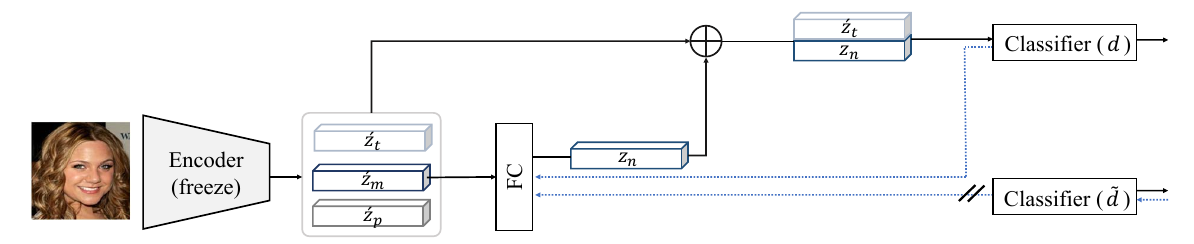
\includegraphics[width=0.75\linewidth]{figures/readme-downstream.png}
    \caption{%
        Downstream classification network of FD-VAE. Source: adapted from Park~\emph{et al.}~\cite{park2020readme}.
    }
    \label{fig:downstream}
\end{figure}

% ----------------------------------------------------------------
\section{Datasets}
\label{sec:readme-datasets}
% ----------------------------------------------------------------

\paragraph{CelebA.}
The CelebA dataset~\cite{liu2015celeba} consists of approximately 200\,000 celebrity face images,
each annotated with 40 binary attributes. The authors consider four (protected, target) attribute
pairs drawn from the attributes \textit{male} (M), \textit{young} (Y), \textit{attractive} (A),
\textit{wavy hair} (W), and \textit{big nose} (B):
\[
    (\text{M},\,\text{A}), \quad (\text{M},\,\text{W}), \quad (\text{Y},\,\text{A}), \quad (\text{Y},\,\text{B}).
\]

\paragraph{UTK Face.}
The UTK Face dataset~\cite{zhang2017utkface} contains face images spanning a wide age range,
annotated for age, ethnicity, and gender. Gender is used as the protected attribute, while ethnicity
(binarised into Caucasian vs.\ others) and age (binarised into young vs.\ older than 35) serve as
target attributes. The training split is constructed to be \emph{imbalanced} between the protected
and target attributes, creating a realistic fairness challenge; the validation and test sets are
balanced.

% ----------------------------------------------------------------
\section{Experimental Results}
\label{sec:readme-results}
% ----------------------------------------------------------------

Table~\ref{tab:celeba-results} and Table~\ref{tab:utk-results} present the classification results on
CelebA and UTK Face datasets, respectively, comparing FD-VAE against four baselines: a plain VAE
(no fairness consideration), $\beta$-VAE, FactorVAE, and FFVAE. For each dataset the baseline
methods are evaluated with the same 60-dimensional representation to ensure a fair comparison.

\subsection{Results on CelebA}

\begin{table}[htbp]
    \centering
    \caption{%
        Classification results on the CelebA dataset. M = male, Y = young, A = attractive,
        W = wavy hair, B = big nose. PA = protected attribute, TA = target attribute.
        $\downarrow$ indicates lower is better (fairer); $\uparrow$ indicates higher is better.
        Bold entries indicate the best result in each column. Source: Park~\emph{et al.}~\cite{park2020readme}.
    }
    \label{tab:celeba-results}
    \small
    \setlength{\tabcolsep}{5pt}
    \begin{tabular}{lllcccc}
        \toprule
        \textbf{Method} & \textbf{TA} & \textbf{PA} &
        \textbf{Equal Opp.~$\downarrow$} & \textbf{Eq.\ Odds~$\downarrow$} &
        \textbf{Acc.~$\uparrow$} & \textbf{Eq.\ Acc.~$\uparrow$} \\
        \midrule
        VAE             & A & M & 27.2 & 28.7 & 70.6 / 65.3 & --- \\
        $\beta$-VAE     & A & M & 21.1 & 22.1 & 68.7 / 64.6 & --- \\
        FactorVAE       & A & M & 20.7 & 23.4 & 69.0 / 64.9 & --- \\
        FFVAE           & A & M & 17.7 & 17.5 & 62.7 / 59.5 & --- \\
        \textbf{FD-VAE (Ours)} & A & M & \textbf{1.3} & \textbf{4.9} & 64.1 / 63.5 & --- \\
        \midrule
        VAE             & W & M & 47.1 & 33.4 & 73.0 / 59.0 & --- \\
        $\beta$-VAE     & W & M & 35.4 & 15.3 & 70.7 / 57.3 & --- \\
        FactorVAE       & W & M & 38.8 & 28.8 & 71.0 / 58.0 & --- \\
        FFVAE           & W & M & 21.1 & 15.4 & 67.7 / 54.3 & --- \\
        \textbf{FD-VAE (Ours)} & W & M & \textbf{13.4} & \textbf{8.9}  & 66.1 / 52.9 & --- \\
        \midrule
        VAE             & A & Y &  9.7 & 11.3 & 70.9 / 69.6 & --- \\
        FFVAE           & A & Y &  8.0 &  8.2 & 64.2 / 62.9 & --- \\
        \textbf{FD-VAE (Ours)} & A & Y & \textbf{3.7} & \textbf{1.9} & 65.5 / 66.0 & --- \\
        \midrule
        VAE             & B & Y & 17.0 & 19.2 & 67.2 / 64.0 & --- \\
        FFVAE           & B & Y &  5.3 &  8.5 & 63.0 / 58.2 & --- \\
        \textbf{FD-VAE (Ours)} & B & Y & \textbf{1.2} & \textbf{1.5} & 63.9 / 57.7 & --- \\
        \bottomrule
    \end{tabular}
\end{table}

The results are striking. On the (M, A) pair, FD-VAE reduces the equal opportunity gap from
FFVAE's 17.7\% to just \textbf{1.3\%} --- a reduction of 16.4 percentage points. Similarly, the
equalized-odds gap falls from 17.5\% to \textbf{4.9\%}. Across all four attribute pairs on CelebA,
FD-VAE consistently outperforms FFVAE by large margins on both fairness metrics while maintaining
comparable accuracy (within 1--2\% of FFVAE on equalized accuracy). This confirms that the
three-way disentanglement preserves more discriminative signal for the target task than the simpler
two-way split of FFVAE.

\subsection{Results on UTK Face}

\begin{table}[htbp]
    \centering
    \caption{%
        Classification results on the UTK Face dataset. G = gender (protected),
        E = ethnicity (target), A = age (target).
        $\downarrow$ = lower is better; $\uparrow$ = higher is better.
        Bold = best result. Source: Park~\emph{et al.}~\cite{park2020readme}.
    }
    \label{tab:utk-results}
    \small
    \setlength{\tabcolsep}{5pt}
    \begin{tabular}{lllcccc}
        \toprule
        \textbf{Method} & \textbf{TA} & \textbf{PA} &
        \textbf{Equal Opp.~$\downarrow$} & \textbf{Eq.\ Odds~$\downarrow$} &
        \textbf{Acc.~$\uparrow$} \\
        \midrule
        VAE         & E & G & 16.1 & 17.4 & 65.2 \\
        $\beta$-VAE & E & G & 12.7 & 12.1 & 60.1 \\
        FactorVAE   & E & G & 12.1 & 12.9 & 59.4 \\
        FFVAE       & E & G &  9.8 &  9.1 & 59.7 \\
        \textbf{FD-VAE} & E & G & \textbf{2.3} & \textbf{1.1} & 60.3 \\
        \midrule
        VAE         & A & G & 24.6 & 29.8 & 60.7 \\
        $\beta$-VAE & A & G & 17.1 & 20.8 & 54.3 \\
        FactorVAE   & A & G & 23.2 & 27.1 & 54.6 \\
        FFVAE       & A & G & 13.6 & 17.2 & 54.5 \\
        \textbf{FD-VAE} & A & G & \textbf{2.0} & \textbf{2.9} & 54.1 \\
        \bottomrule
    \end{tabular}
\end{table}

On UTK Face, FD-VAE achieves 2.3\% and 2.0\% equal opportunity for the ethnicity and age
classification tasks respectively --- reductions of roughly 7 to 11 percentage points over FFVAE
with no meaningful drop in accuracy. This demonstrates that the improvement generalises across
different datasets and protected-attribute types.

% ----------------------------------------------------------------
\section{Summary}
\label{sec:readme-summary}
% ----------------------------------------------------------------

The README framework makes three distinct contributions to fair representation learning, which we
briefly recap here before connecting them to the broader context of the report:

\begin{description}
    \item[Three-way latent disentanglement.] By introducing the Mutual Attribute Latent as a
          third subspace alongside the target and protected attribute latents, README avoids the
          information leak that afflicts two-way disentanglement approaches. This single design
          change enables a far cleaner separation of attribute-specific information.

    \item[Explicit decorrelation via adversarial supervision.] The decorrelation loss goes beyond
          generic disentanglement: it provides direct supervision via $L_\text{CLS}$ to assign
          correct information to each subspace, and adversarially removes unwanted cross-information
          via $L_\text{ADV}$. This two-pronged approach is shown in the ablation study to be the
          decisive factor for fairness.

    \item[Novel equalized accuracy metric.] By proposing an accuracy metric that weights all
          group--outcome combinations equally, README provides the community with a tool that is
          immune to dataset imbalance, making comparisons across skewed benchmarks more meaningful.
\end{description}

The experimental results on CelebA and UTK Face demonstrate that FD-VAE outperforms all prior
methods by substantial margins on standard fairness metrics (equal opportunity, equalized odds),
while achieving comparable accuracy. The framework lays the groundwork for the application we
explore in Chapter~\ref{ch:cvar_deepfake}: extending fairness-aware representation learning to the
more challenging problem of deepfake detection.

\vspace{2em}
% ---- Chapter Bibliography Note --------------------------------
\noindent\textit{The primary reference for this chapter is Park~\emph{et al.}, ``README: REpresentation
learning by fairness-Aware Disentangling MEthod,'' arXiv:2007.03775v1, 2020. All tables and figures
are adapted from this paper.}